\documentclass[12pt, a4paper]{article}
\setlength{\parindent}{0pt}
\usepackage{amsmath}
\usepackage{amsthm}
\usepackage{amssymb}
\usepackage{graphicx}
\usepackage[a4paper, portrait, margin=1in]{geometry}

\graphicspath{.}

% i like the black square better.
\renewcommand{\qedsymbol}{$\blacksquare$}
%\renewcommand{\implies}{\Rightarrow}

\newcommand{\N}{\mathbb{N}}
\newcommand{\ddr}{\frac{d}{dr}}

\newtheorem{theorem}{Theorem}

% let's begin
\begin{document}

\textbf{(Q1)}

For clarity, we redefine the height and radius of the cone as $H$ and $R$
respectively, and the height and radius of the inscribed cylinder to be $h$ and $r$.

\begin{center}
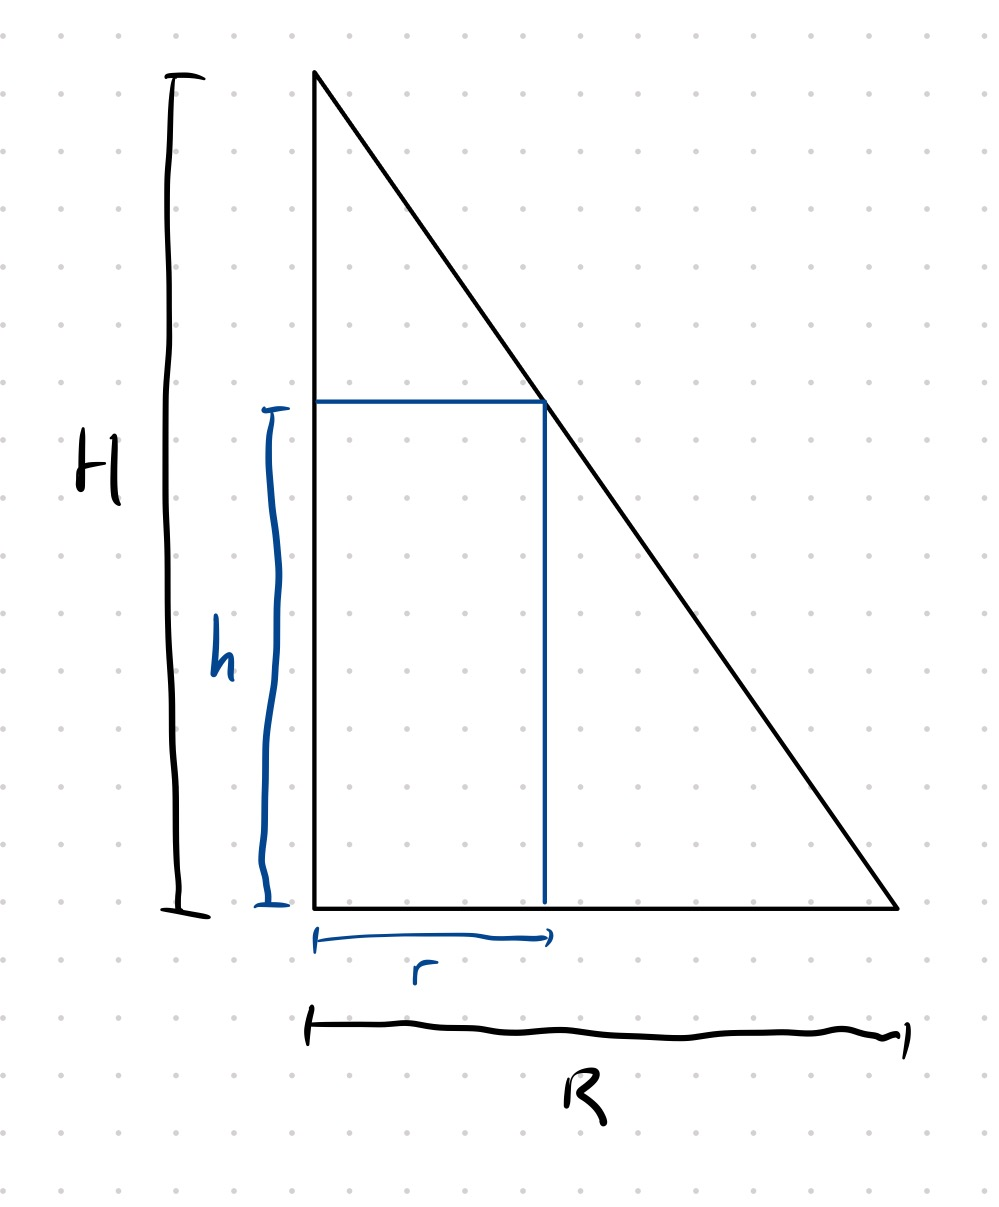
\includegraphics[width=10cm]{q1_cone.JPG}
\end{center}

From the above figure, we observe from similar triangles that:

\begin{align}
    \frac{H}{R} & = \frac{H - h}{r}\\ & = \frac{h}{R - r}
\end{align}

We will use (2) for this solution.

From the formula for volume of a cylinder, we define the volume $V_c$ of a
given cylinder inscribed within the cone with:
\[
    V_c = \pi r^2h
\]

Since $h = \frac{H(R - r)}{R}$, we have
\[
    V_c = \frac{\pi}{R}r^2 H(R - r)
\]

We aim to find the maximum for $V_c$, so we need to find $r$
for which this function is at a maximum.

\newpage

Differentiating it and then solving for zero, we have
\begin{align*}
    \frac{2\pi}{R}rH(R - r) + \frac{\pi}{R}r^2(-H) & = 0\\
    2Rr - 3r^2 & = 0\\
    r(2R - 3r) & = 0\\
    r = 0, \;\; r & = \frac{2R}{3}
\end{align*}

Since $r$ cannot be 0, $\frac{2R}{3}$ is the only possible answer.
Substituting this value of $r$ into $V_c$, we have:

\begin{align*}
    V_c & = \frac{\pi}{R}\left(\frac{2R}{3}\right)^2 \cdot H \left(R - \frac{2R}{3}\right)\\
    & = \frac{4 \pi R}{9} \cdot \frac{HR}{3}\\
    & = \frac{4}{3}\pi R^2 H
\end{align*}

\end{document}